
\section{\engt{Lesson 3: LED Cube Construction} \nedt{Les 3: LED Cube constructie}}

\subsection{\engt{Layout breadboard}  \nedt{Opstelling schakelbord}}

\eng{We have all the necessary basis to start with making our Fe Cube. We start with putting all components on the breadboard. Then we test it with a program which is our previous RGB LED sketch adapted to the cube. Only when we have verified all works will we start the actual construction.

So, put following components in front of you:
\begin{enumerate}
 \item Your breadboard
 \item 9 RGB-LED (we assume common cathode in the following)
 \item 3 NPN (2N3904 normally)
 \item 9 220 $\Omega$ resistors
 \item many wires.
\end{enumerate}
First, put the RGB-LED on the board, connect the color pins with each other via wires, and connect the common cathode via a resistor to another line, see Fig.~\ref{f:lesson3_bb1}.

Connect then the resistors to pins 1 to 9. These are the pins that will feed the LED. So for a common cathode, these pins on \ardo{HIGH} will make the LED burn. Put the 3 NPN on the board. The color wire goes to the Emitter side (-) of the NPN for common cathode LED. The Colector side (+) goes to the Volt line of your breadboard. The Volt line of the breadboard goes to a 5V pin on the Arduino.

The Base leg of the NPN will control if the NPN junction is open or not. We will use pins 10, 11, 12 to control this. Your entire wiring should look like Fig.~\ref{f:lesson3_bb2}.
}

\ned{We hebben alles gezien om aan onze Fe Kubus te beginnen. We starten met alle componenten op het schakelbord te zetten. Dan testen we de schakeling met een programma die onze vorige RGB LED schets is aangepast voor de kubus. Alleen als we zeker zijn dat alles werkt zullen we de effectieve constructie doen.

Plaats dus de volgende componenten voor jou:
\begin{enumerate}
 \item Jouw schakelbord
 \item 9 RGB-LED (we veronderstellen gemeenschappelijke kathode in wat volgt)
 \item 3 NPN (2N3904 normaal)
 \item 9 220 $\Omega$ weerstanden
 \item veel draden.
\end{enumerate}
Begin met de RGB-LED op je bord te zetten, verbindt de kleurpinnen met elkaar via draden, en connecteer de gemeenschappelijke kathode via een weerstand naar een andere lijn op je bord, zie Fig.~\ref{f:lesson3_bb1}.

Verbind nu de weerstanden met pinnen 1 tot 9. Deze pinnen zullen de LED van stroom voorzien. Dus, voor een gemeenschappelijke kathode zullen we deze pinnen op \ardo{HIGH} zetten om de LED te doen branden. Plaats dan de 3 NPN op het bord. De draden van een kleur gaan naar de Emitter zijde (-) van de NPN voor gemeenschappelijke kathode LEDs. De Collector zijde (+) gaat naar de Voltage lijn op je schakelbord. Deze Voltage lijn gaat dan naar een 5V pin op de Arduino.

Het Basis been van de NPN zal bepalen of de NPN junctie open is of niet. We zullen pinnen 10, 11, 12 gebruiken voor dit been. Je volledige schakeling zou er moeten uitzien als Fig.~\ref{f:lesson3_bb2}.
}

\begin{figure}
  \centering
  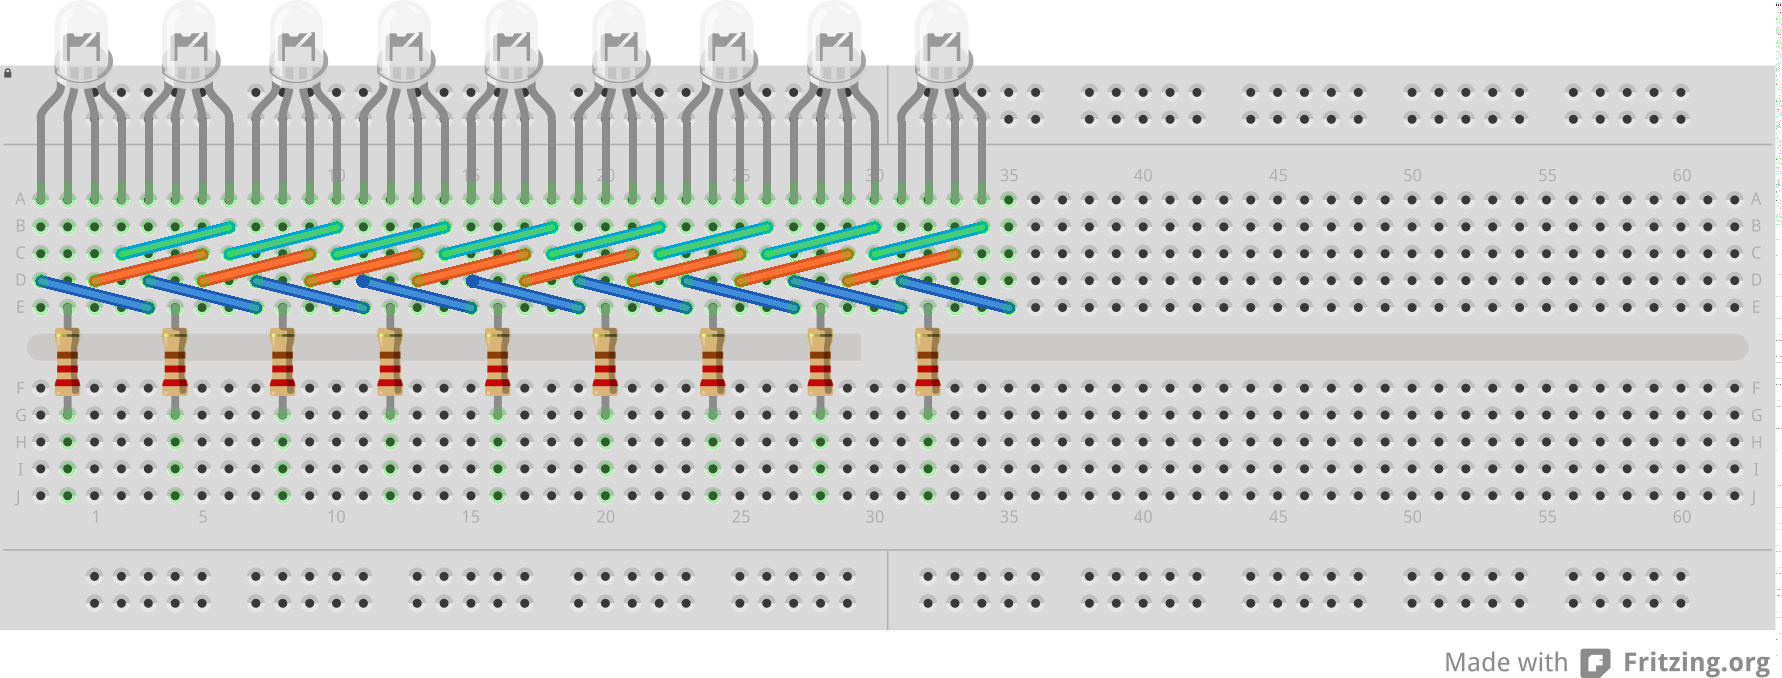
\includegraphics[width=11cm]{img/05_fecube_01_bb.png} 
\caption{\engt{Put the 9 LED on the board. Connect all equal colors to each other. The common cathode or anode goes with a 220 $\Omega$ resistor to a new line} \nedt{Plaats de 9 LED op het bord. Connecteer alle gelijke kleuren met elkaar. De gemeenschappelijke kathode of anode gaat met een 220 $\Omega$ weerstand naar een nieuwe lijn.}}
\label{f:lesson3_bb1}.
\end{figure}
%
\begin{figure}
  \centering
  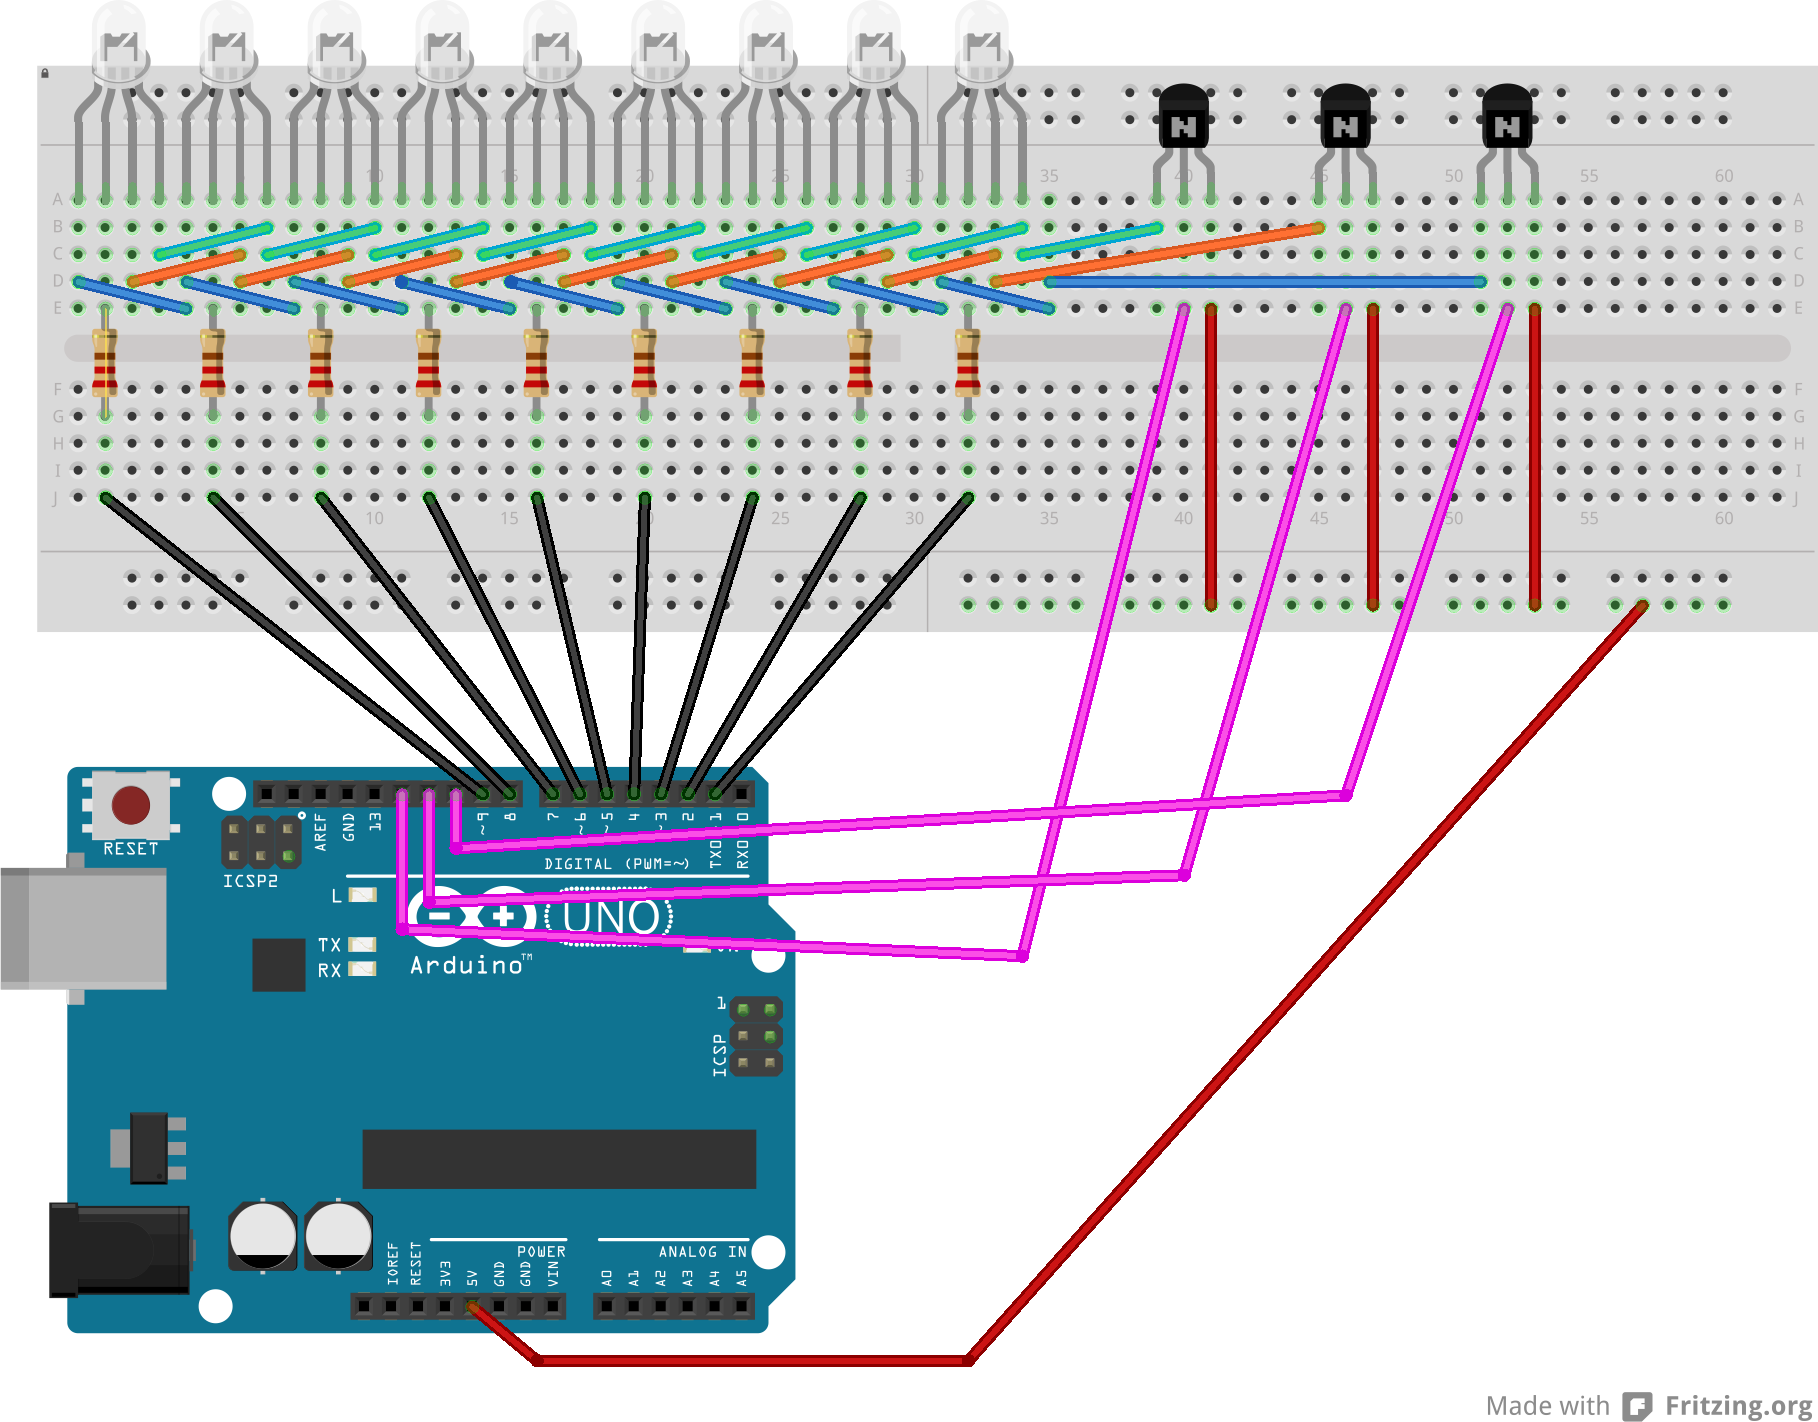
\includegraphics[width=11cm]{img/05_fecube_02_bb.png} 
\caption{\engt{Connect the resistors to pins 1 to 9. The colors go via an npn to the GND (cathode) or 5V (anode). Pins 10, 11, 12 go to the NPN to control the colors.} \nedt{Verbind de weerstanden met pinnen 1 tot 9. De kleuren gaan via een npn naar de GND (kathode) of 5V (anode). Pinnen 10, 11, 12 gaan naar de NPN om de kleuren te schakelen.}}
\label{f:lesson3_bb2}
\end{figure}

\subsection{\engt{Testing breadboard Fe Cube}  \nedt{Schakelbord Fe Cube uittesten}}

\eng{We will only verify we can make the breadboard Fe Cube work. For this we adapt our RGB sketches. We will make a movie showing 1 minute a random color, then 4 seconds red, then 4 seconds green, then 4 seconds blue, then smooth transitions for 1 minute.

This means we need all the shots we created for the RGB LED in the previous lesson, and need to create an adapted \ardo{movie} function to connect the shots as we want. We also need to change the start so that instead of only one led pin, we start up 9 led pins. 

In our previous script, we had ledR, ledG, ledB, which are easy to understand names. The led was called led1, so we could use led1 to led9. This is not very helpfull if you want to program certain light effects. So, let's give them better names. We have a top layer (T), and a bottom (B) layer, and a single LED in the middle. Then we can divide the cube in a left (L) and right (R), and in a front (F) and an aft (A). So, let's call the LEDs:
\begin{enumerate}
\item ledTLF
\item ledTLA
\item ledTRF
\item ledTRA
\item ledBLF
\item ledBLA
\item ledBRF
\item ledBRA
\item ledMID
\end{enumerate}
Open Code \ref{c:l2_d}, and save it under a new name. The changes needed are first defining all the pins:
}

\ned{TODO}

\inputard{\string"../sketches/Fe_cube_03_cube_test1/Fe_cube_03_cube_test1.ino\string"}{5}{11}

\eng{Next we need to define in \ardo{setup} that these are digital output pins, so:}


\ned{TODO}

\inputard{\string"../sketches/Fe_cube_03_cube_test1/Fe_cube_03_cube_test1.ino\string"}{15}{24}

\eng{We test the cube as a single LED, so all LED are on, or all LED are off. Hence, instead of setting only led1 on, we write a function to put all LED on, and put that in \ardo{show\_subframe\_color}}
\ned{TODO}

\inputard{\string"../sketches/Fe_cube_03_cube_test1/Fe_cube_03_cube_test1.ino\string"}{209}{211}
and with that function for setting the pins \textbf{on} sending a LOW signal, as we are connected to the LED cathode (-)
\inputard{\string"../sketches/Fe_cube_03_cube_test1/Fe_cube_03_cube_test1.ino\string"}{230}{243}

\eng{Finally, we need to update the \ardo{movie} function so that it would do what we want. So this function needs to be}
\ned{TODO}

\inputard{\string"../sketches/Fe_cube_03_cube_test1/Fe_cube_03_cube_test1.ino\string"}{108}{142}


\engo{\begin{doE}
      \textbf{One LED}. To test that a single LED does indeed not shine brighter when it is alone, change the \ardo{all\_led\_on} code so that only one LED has power.
     \end{doE}
}
\nedo{\begin{doN}
      \textbf{\'E\'en LED}. Om te testen dat een LED alleen inderdaad niet helderder brandt, wijzig de \ardo{all\_led\_on} functie zodat maar \'e\'en LED aan is.
     \end{doN}
}


\subsection{\engt{Construction}  \nedt{Constructie}}
\eng{We verified all is working, time to construct the cube. For this we will take components of our breadboard, and solder the connections in a FE Cube form.
We call our cube the Fe Cube because it is organized as the Iron metal lattice. Solid iron has a specific structure which is present in the Atomium building in Brussels. 
}

\ned{TODO}

\section{\engt{Lesson 4: Fire up the LED Cube} \nedt{Les 4: De LED Cube gebruiken}}

\subsection{\engt{Testing the Fe Cube} \nedt{De Fe Cube testen}}
\eng{You finished now constructing the cube. We need to test if all lights are working. Start with the same sketch you used for the breadboard cube. If you connect everything correctly, it should just work. 

If things are not working, you have some extra soldering to do: replace a blown out LED, make connections stronger, ... . Don't give up now. These are the last construction problems of your led cube.}
\ned{TODO}

\subsection{\engt{Generic patterns ... and a snake} \nedt{Algemene patronen ... en een slang}}

\eng{
Let us create a generic shot that can load patterns. Like that we can write down a pattern, and pass it to this shot. The first pattern we want to make is the snake patters: a single light that jumps from LED to LED in the three base colors.

We need to define the data structure of a pattern. What needs to be in a pattern?
\begin{enumerate}
 \item We need for 9 LED what color they must have. A color is a RGB value like (13,50,2), so in base 64. That is, we need 27 numbers.
 \item We need to know how long to hold this pattern before moving to the next pattern. So, we need an extra number for the milliseconds to hold the pattern.
\end{enumerate}
Therfore, a pattern will look like :\newline
$\{$R1,G1,B1, R2,G2,B2, R3,G3,B3, R4,G4,B4, R5,G5,B5, R6,G6,B6, R7,G7,B7, R8,G8,B8, R9,G9,B9, duration$\}$\newline

The order of the LEDS in this pattern will be ledTLF, ledTLA, ledTRF, ledTRA, ledBLF, ledBLA, ledBRF, ledBRA, ledMID. If a shot consists of 20 patterns, we create a single large array with all the patterns, one after the other. As Arduino code is not that clever, we need to know somehow what the last pattern is. We could count and pass this number of patterns, but that will quickly lead to an error. Easier is to finish the list with a dummy pattern with duration 0. If we read this 0, we know the pattern is finished. 

In our code, our movie function will read one pattern at a time, and then use the fixed\_pattern function to display the pattern.
}
\ned{TODO}

\eng{
The code is given in Code \ref{c:ledcube_snake}.
}

\ned{TODO}

\begin{code}\label{c:ledcube_snake}
 \ \newline
\inputardfull{\string"../sketches/Fe_cube_03_cube_pattern/Fe_cube_03_cube_pattern.ino\string"}
\end{code}

%\begin{code}\label{c:ledcube_smooth}
% \ \newline
%\inputardfull{\string"sketches/Fe_cube_04_common_kathodeRGB_cube_smoothrandom/Fe_cube_04_common_kathodeRGB_cube_smoothrandom.ino\string"}
%\end{code}


